\begin{frame}
\frametitle{Moteur}
\framesubtitle{Dimensionnement}
\begin{description}
\item[Régime permanent]
\item En régime permanent l'accélération est nulle;
\item $Fm - Fr = m \times \overrightarrow{a} = 0$.
\item[Résultats]
\item $P = Cm \times \omega m = 694\frac {rad}{s}  \times 0.02943N = 20.42W$;
\item Vitesse maximale du robot $V = 5\frac{km}{h} = 1.38\frac{m}{s}$.
\end{description}
\end{frame}

\begin{frame}
\frametitle{Moteur}
\framesubtitle{Dimensionnement en tenant compte de l'accélération}
\begin{itemize}
\item Pour simplifier les calculs on suppose qu'on atteint la vitesse du régime, c'est-à-dire 1.38m/s en 1s;
\item $Fm - Fr = m \times \overrightarrow{a} = 10kg \times 1.38\frac{m}{s^{2}} = 13.8N$;
\item $Fm = Fr + 13.8N = 13.8 + 17.715 = 28.5N$ ;
\item $Croue = Fr \times r = 28.5N  \times 0.04m = 1.14Nm$, $r = 0.04m$ rayon de la roue ;
\item $Cmoteur = \frac {Croue}{20} = 57mNm$;
\item $P = Cm \times Wm = 0.057mNm \times 694\frac{rad}{s} = 39.7W$;
\item $2 moteurs \rightarrow 20 Watts par moteur$.
\end{itemize}
\end{frame}

\begin{frame}
\frametitle{Moteur}
\begin{figure}[!ht]
	\centering
	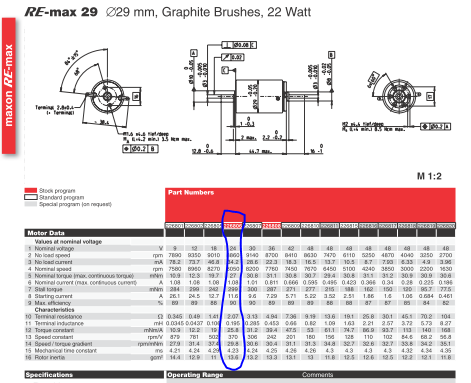
\includegraphics[scale=0.7]{Moteur.PNG}
	\caption{Moteur}
\end{figure}
\end{frame}

\begin{frame}
\frametitle{Moteur}
\begin{figure}[!ht]
	\centering
	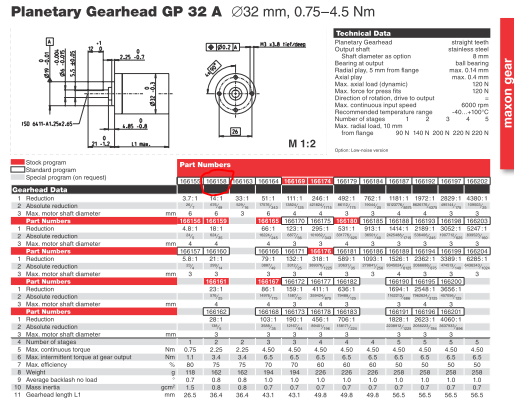
\includegraphics[scale=0.6]{Gearhead.PNG}
	\caption{Gearhead}
\end{figure}
\end{frame}

\begin{frame}
\frametitle{Moteur}
\begin{figure}[!ht]
	\centering
	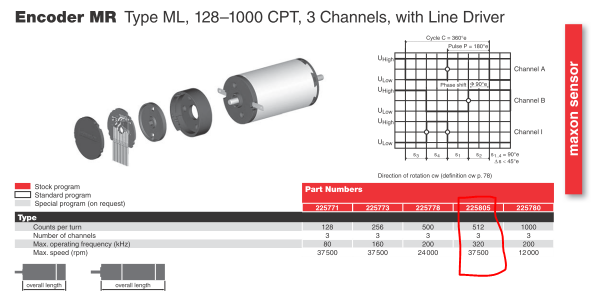
\includegraphics[scale=0.6]{Encoder.PNG}
	\caption{Encoder}
\end{figure}
\end{frame}

\begin{frame}
\frametitle{Driver}
\end{frame}